\label{ssec:webgui}
In order to interact with the robot, apart from speech, we have designed a web-based \gls{gui}. This interface uses HTML5\footnote{\url{https://github.com/tue-robotics/tue_mobile_ui}} with the Robot API written in Javascript and we host it on the robot itself.
%This allows multiple users on different platforms (\eg\ Android, iOS) to access functionalities of the robot. The interface is implemented in JavaScript with AngularJS and it offers a graphical interface to the Robot API\footnote{\url{https://github.com/tue-robotics/robot-api}} which exposes all the functionality of the robot.
%\begin{figure}[h]
%    \centering
%	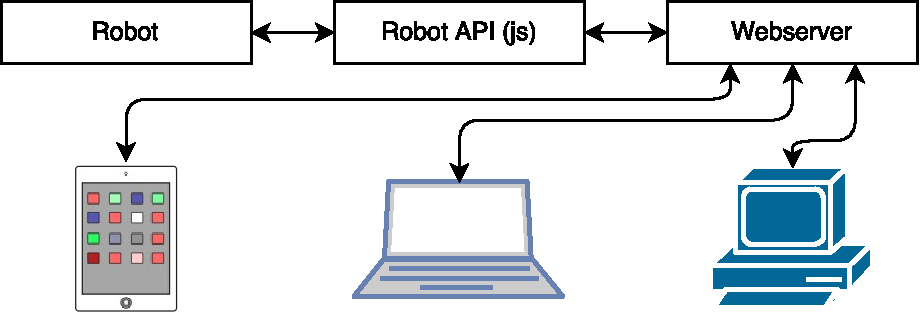
\includegraphics[width=0.9\linewidth]{Figures/webgui_architecture}
%    %\vspace{-0.5em}
%	\caption{
%		Overview of the WebGUI architecture.
%		A webserver that is hosting the \protect\gls{gui} connects this %Robot API to a graphical interface that is offered to multiple clients on %different platforms.}
%	\label{fig:webgui_architecture}
%\end{figure}
%Figure~\ref{fig:gui_actions} gives an example of various user interactions that are possible with the \gls{gui} and the different commands that can be given to the robot while interacting with the virtual scene.

\begin{figure}[H]
	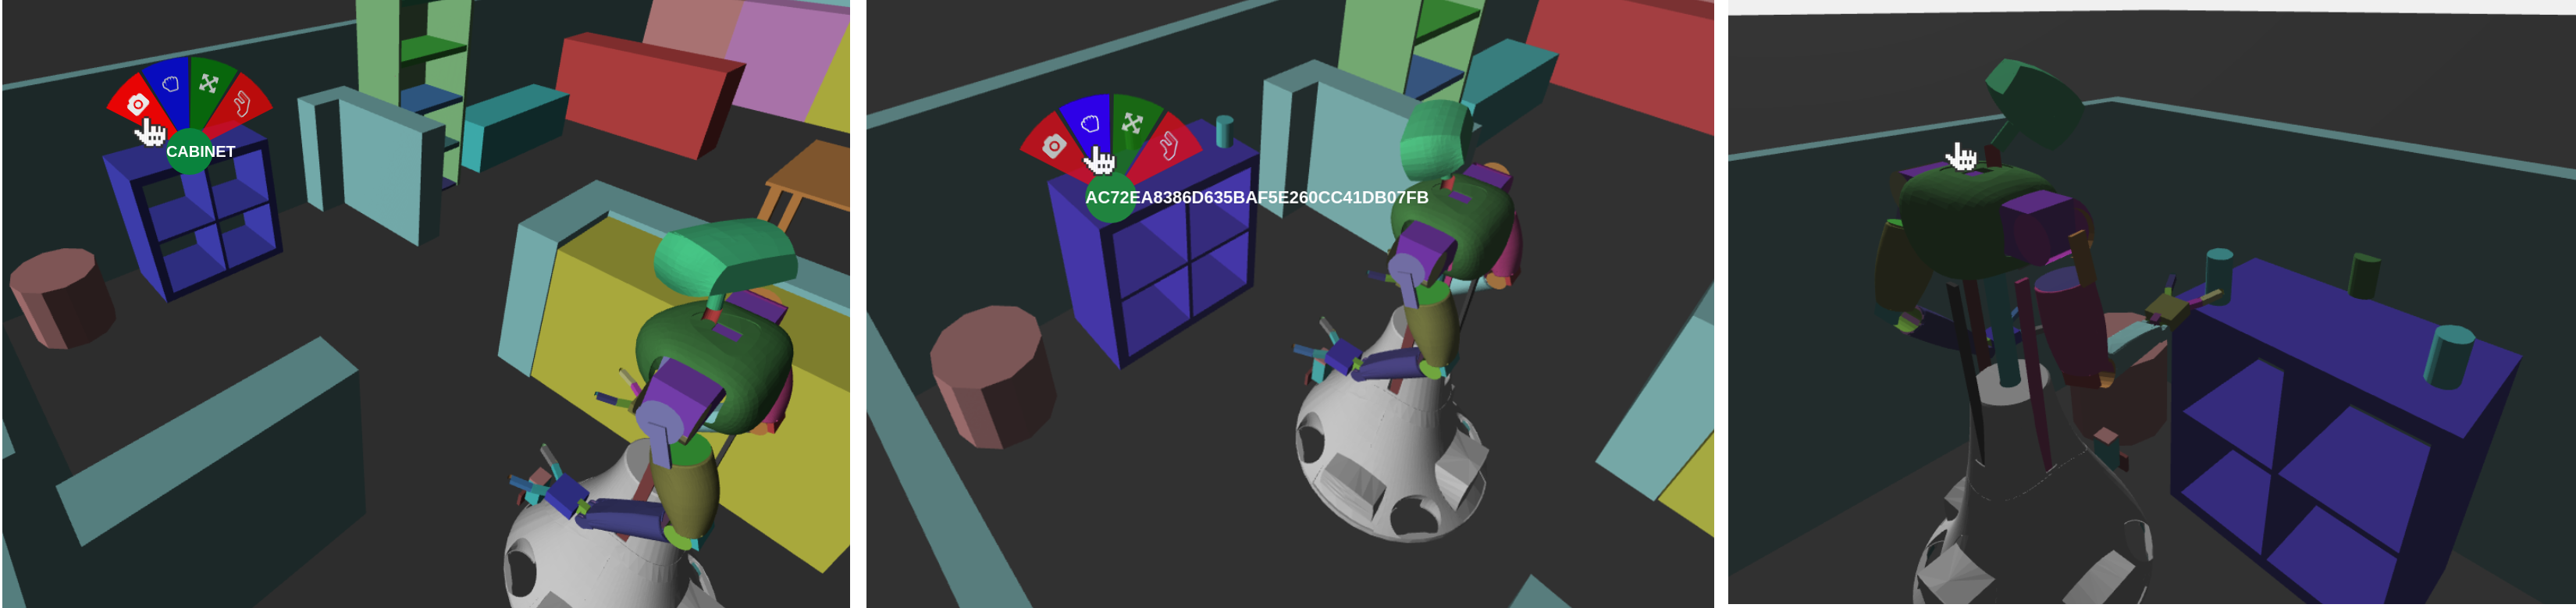
\includegraphics[width=\linewidth]{Figures/gui_actions}
	\caption{
		Illustration of the 3D scene of the WebGUI with AMIGO.
		User can long-press objects to open a menu from which actions on the object can be triggered
%		Users can interact with use of the menu that appears when long pressing an object in the scene.
%		On the left figure, the user commands the robot to inspect the selected object, which is the `cabinet'.
%		When the robot has inspected the `cabinet', it has found entities on top of it.
%		In the middle figure a grasp command is given to the robot to pick up an object from the cabinet.
%		The last figure show the robot executing that action.
		}
	\label{fig:gui_actions}

\end{figure}
%Figure \ref{fig:webgui_architecture} gives an overview of the connections between these components and 
Figure \ref{fig:gui_actions} represents an instance of the various interactions that are possible with the Robot API.
